%CHAPTER
\chapter{Patent}
\todo{todo}
základní informace + uložiště dat + info o zdrojích (patentové úřady atp) \newline
\section{Patent vs Užitný vzor}
\section{Patent vs Průmyslový vzor}
\section{Patent vs Ochranná známka}
\section{Patent vs Autorská práva}


%%%%%%%%%%%%%%%%%%%%%%%%%%%%%%%%%%%%%%%%%%%%%%%%%%%%%%%%%%%%

%CHAPTER
\chapter{Databáze}

Termín databáze označuje organizovanou kolekci strukturovaných informací nebo dat, která jsou typicky ukládána elektronicky v počítačovém systému. Data / informace lze nazvat jako fakta vztahující se k libovolnému uvažovanému objektu. Typický příklad objektu je člověk, jehož fakta jsou: jméno, věk, výška, váha a mnoho dalších \cite{guru99Database}.\newline

\section{Systém řízení báze dat}
Pro správu dat v databázi a její řízení je potřeba komplexní software, který se nazývá \textbf{Systém Řízení Báze Dat} (SŘBD, anglicky \gls{DBMS}). SŘBD slouží jako interface mezi samotnou databází a koncovým uživatelem (může být i program), umožňující jak vytěžování a aktualizaci dat, tak i možnosti nastavení záloh a jiných administrativních operací \cite{OracleDB}. V dnešním světe existuje několik různých \gls{DBMS} (například Relační \gls{DBMS}, Objektově-orientované \gls{DBMS}).
\begin{figure}[h!]
\centering
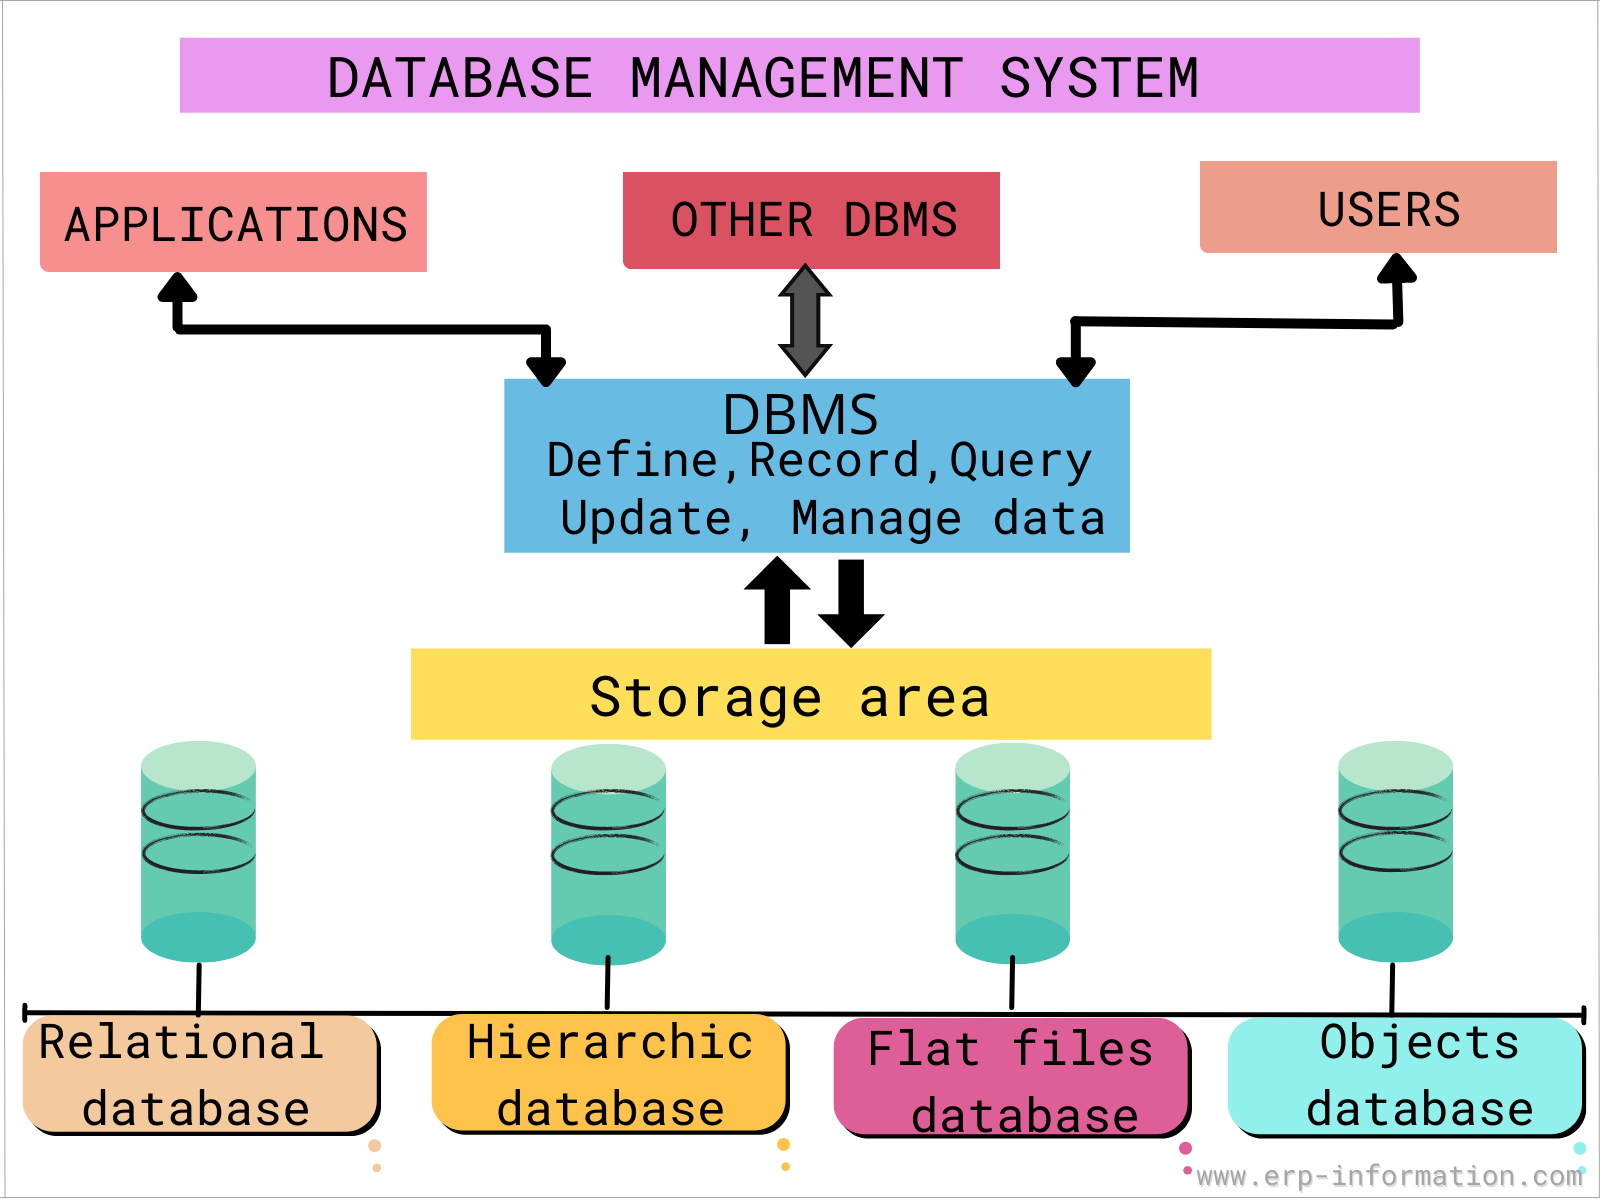
\includegraphics[width=10cm]{img/databaze/dbms}
\caption{Systém řízení báze dat}
\label{fig:dbms}
\end{figure}

\section{Komponenty databáze}
Všechny databáze sestávají z pěti základních komponent, nehledě na použitý typ databáze \cite{TechTargetDB, guru99Database}:
\begin{itemize}
\item \textbf{Hardware} - Fyzické stroje (počítače, servery, pevné disky, ...) na kterých běží databázový software.
\item \textbf{Software} - Databázový software poskytuje uživateli / programu kontrolu nad databází. Zahrnuje to samotný databázový software, operační systém, software pro správu sdílení dat mezi uživately a programy pro přístup k datům v databázi.
\item \textbf{Data} - Nezpracované a neorganizované fakty, které je potřeba zpracovat. Administrátor databáze organizuje tyto data a dává jim význam. Data se obecně skládají hlavně z faktů, observací, percepcí, čísel, znaků a mnoho dalších.
\item \textbf{Jazyk} - Typický příklad použití jazyku je přístup k datům, přidávání nových dat, úpravu již existujících dat z databáze. Uživatel / program napíše specifické příkazy v jazyku pro přístup k datům (Database Access Language) a tyto příkazy následně pošle databázi ke zpracování. Více viz kapitola č. \ref{sec:jazyky}.
\item \textbf{Procedury} - Procedura obsahuje předpřipravený seznam příkazů, které se následně vykonávají po zavolání dané procedury. 
\end{itemize}

\section{Jazyky} \label{sec:jazyky}
Databázové jazyky, jinak známé jako dotazovací jazyky, jsou klasifikací programovacích jazyků, které se používají k definování a přístupu k databázím. Pomocí těchto jazyků dokáže uživatel získávat nebo spravovat data v databázích. V dnešní době se jazyky (například \gls{SQL}) mohou skládat ze čtyř podjazyků, kdy každý slouží k jinému účelu v rámci vykonávání příkazů \cite{indeedDBLanguage, begginersBookDBLanguage}:
\begin{itemize}
\item \textbf{Data definition language} (DDL) - DDL umí vytvářet jednotlivé komponenty databázového schématu (tabulky, soubory, indexy, ...), které tvoří strukturu reprezentující organizaci dat v databázi. Dostupné příkazy pro jazyk DDL:
	\begin{itemize}
	\item \textbf{CREATE} - Vytvoření nového objektu (tabulka, index, ...).
	\item \textbf{ALTER} - Změna struktury objektu.
	\item \textbf{DROP} - Smazání objektu.
	\item \textbf{RENAME} - Změna názvu objektu.
	\item \textbf{TRUNCATE} - Smazání podobjektů v objektu (například záznamy v tabulce).
	\end{itemize}
\item \textbf{Data manipulation language} (DML) - DML slouží pro manipulaci s daty, které se nachází v již existující databázi. Dostupné příkazy pro jazyk DML:
	\begin{itemize}
	\item \textbf{SELECT} - Získání záznamů (dat) z tabulky.
	\item \textbf{INSERT} - Vložení nového záznamu (dat) do tabulky.
	\item \textbf{UPDATE} - Úprava existujícího záznamu v tabulce.
	\item \textbf{DELETE} - Smazání záznamu z tabulky.
	\end{itemize}
\item \textbf{Data control language} (DCL) - Pomocí DCL lze kontrolovat přístupy a práva k datům, které jsou uloženy v databázi. Uživateli lze nastavit práva k jednotlivým DML příkazům nad tabulkama / procedurama (například uživatel bude mít přístup pouze k příkazu SELECT nad tabulkou "TABULKA"). Dostupné příkazy pro jazyk DCL:
	\begin{itemize}
	\item \textbf{GRANT} - Přidání práv uživateli nad danou tabulkou / procedurou. 
	\item \textbf{REVOKE} - Odebrání práv uživateli nad danou tabulkou / procedurou.
	\end{itemize}

\item \textbf{Transaction control language} (TCL) - TCL spravuje transakce v databázi. Transakce obsahuje jeden či více DML příkazů nad tabulkama, které se vykonávají po sobě. Všechny příkazy musí být úspěšně provedeny, aby bylo možné transakci označit za úspěšnou. Ukázka jedné transakce viz obrázek č. \ref{fig:tcl_savepoint}. Dostupné příkazy pro jazyk TCL:
	\begin{itemize}
	\item \textbf{COMMIT} - Potvrzení transakce, změny provedené v transakci jsou permanentní a nejdou vzít zpět.
	\item \textbf{ROLLBACK} - Vezme zpět veškerou práci v aktuální transakci. Lze se vrátit na začátek transakce nebo k SAVEPOINTu.
	\item \textbf{SAVEPOINT} - Nastavení bodu v transakci, ke kterému se lze v budoucnu vrátit pomocí ROLLBACK.
	\end{itemize}
\end{itemize}
	\begin{figure}[H]
	\centering
	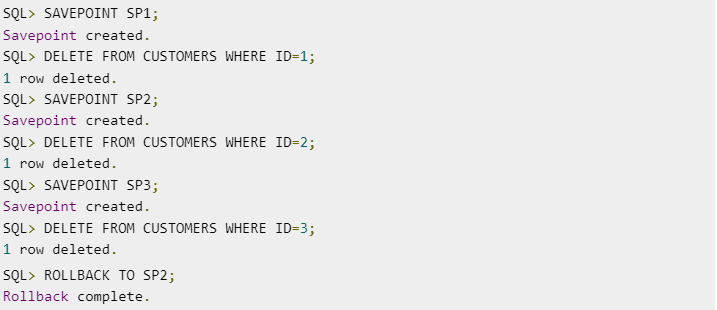
\includegraphics[width=14cm]{img/databaze/tcl_savepoint}
	\caption{Ukázka jedné transakce (bez commitu)}
	\label{fig:tcl_savepoint}
	\end{figure}
\section{Typy databází}
V dnešním světě existuje mnoho různých typů databází. Výběr nejlepšího typu databáze pro konkrétní organizaci závisí na tom, jak organizace zamýšlí data používat. V této kapitole je vypsáno pouze pár typů, protože vznikají stále nové, méně známé typy databází, které jsou tvořeny pro specifické požadavky (například finanční, věděcké) \cite{matillionTypeDB, OracleDB}.
\subsection{Relační databáze}
Název relační databáze pochází ze způsobu, jakým jsou data uložena, a to ve více souvisejících tabulkách. Data v tabulkách jsou uložena v řádcích a sloupcích. Relační databáze jsou velice spolehlivé a podporují všechny čtyři žádoucí vlastnosti databázových transakcí \gls{ACID}. Pro co nejefektivěnjší využití tohoto typu databáze je potřeba ukládat pouze dobře strukturovaná data, pro částečně strukturovaná či nestrukturovaná data je vhodné použít například grafové nebo dokumentově založené databáze. Typické relační databáze jsou například: Microsoft SQL Server, Oracle Database, MySQL. Ukázku relační databáze lze vidět na obrázku č. \ref{fig:db_img_relational}.
	\begin{figure}[H]
	\centering
	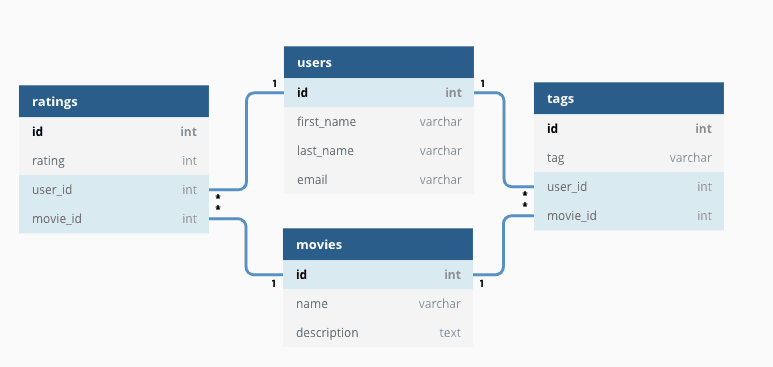
\includegraphics[width=14cm]{img/databaze/relational_db}
	\caption{Ukázka relační databáze}
	\label{fig:db_img_relational}
	\end{figure}
\subsection{Objektově-orientovaná databáze}
Objektově-orientovaná databáze je založena na objektově-orientovaném programování, kdy data a všechny jejich atributy a metody jsou svázány dohromady jako objekt. Stejně jako relační databáze, i objektově-orientované databáze odpovídají standardům \gls{ACID}. Typické příklady jsou například: ObjectStore, Cache, ConceptBase. Ukázku objektově-orientované databáze lze vidět na obrázku č. \ref{fig:db_img_oo}.
	\begin{figure}[H]
	\centering
	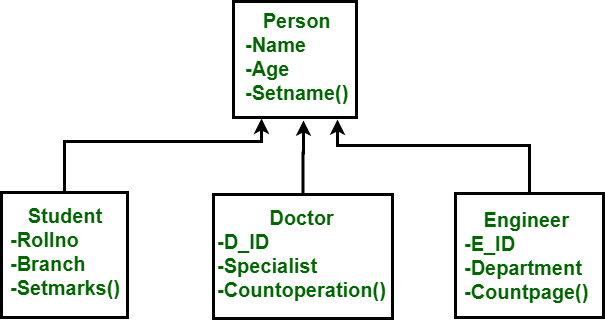
\includegraphics[width=12cm]{img/databaze/oo_db}
	\caption{Ukázka objektově-orientované databáze}
	\label{fig:db_img_oo}
	\end{figure}
\subsection{Cloud databáze}
Cloudová databáze je kolekce dat, strukturovaných nebo nestrukturovaných, která se nachází na soukromé, veřejné nebo hybridní platformě cloud computingu. Stejně jako ostatní cloudové aplikace, cloudové databáze nabízejí flexibilitu a škálovatelnost spolu s vysokou dostupností. Existují dva typy modelů: tradiční a databázový jako služba (DBaaS). Typické příklady jsou: Amazon Web Service, Simtech, Google Cloud Platform. Ukázku cloud databáze lze vidět na obrázku č. \ref{fig:db_img_cloud}.
	\begin{figure}[H]
	\centering
	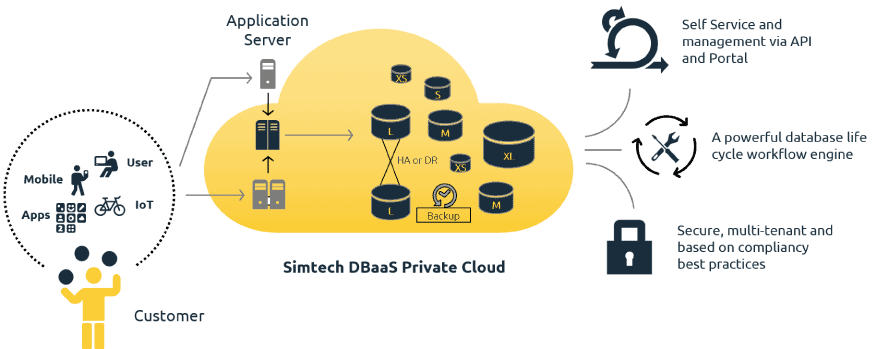
\includegraphics[width=15cm]{img/databaze/cloud_db}
	\caption{Ukázka cloud databáze - databáze jako služba}
	\label{fig:db_img_cloud}
	\end{figure}
\subsection{Distribuovaná databáze}
Distribuovaná databáze je skupina vzájemně propojených databází (dvě a více), které jsou fyzicky rozloženy na různých místech, která jsou spravována systémem správy distribuovaných databází (\gls{DBMS}). V tomto typu systému nejsou data uložena na jednom místě. Při spuštění dotazu se pomocí kolektivní sady webů napříč různými datovými centry spolupracuje na zodpovězení otázky. Typické příklady jsou: Apache Ignite, AWS SimpleDB, FoundationDB. Ukázku distribuované databáze lze vidět na obrázku č. \ref{fig:db_img_distributed}.
	\begin{figure}[H]
	\centering
	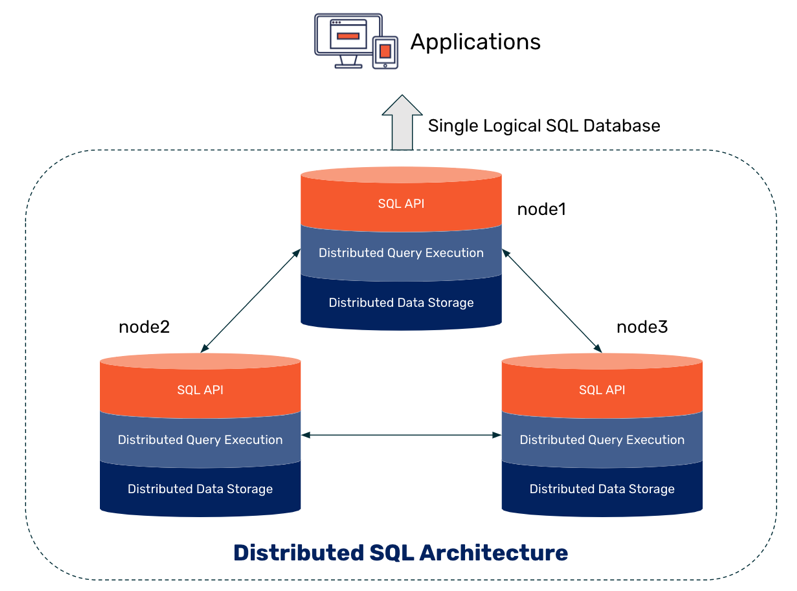
\includegraphics[width=13cm]{img/databaze/distributed_db}
	\caption{Ukázka distribuované databáze}
	\label{fig:db_img_distributed}
	\end{figure}
\subsection{NoSQL databáze}
NoSQL je široká kategorie databází, které nepoužívají \gls{SQL} jako svůj primární jazyk pro přístup k datům. Tyto typy databází jsou také někdy označovány jako nerelační databáze. V NoSQL databázích se pracuje s nestrukturovanými a polostrukturovanými sadami distribuovaných dat. Jednou z výhod je, že vývojáři mohou provádět změny databáze za běhu, aniž by to ovlivnilo aplikace, které databázi používají.
\subsection{Databáze Klíč-Hodnota}
Databáze klíč-hodnota poskytuje nejjednodušší možný datový model. Data jsou uložená jako pár klíč - hodnota ve slovníku / mapě, kdy klíč je indexem. Hodnota může být například celé číslo, řetězec, struktura \gls{JSON} nebo pole. Typické příklady jsou: Redis, Riak, Oracle NoSQL Database. Ukázku databáze klíč-hodnota lze vidět na obrázku č. \ref{fig:db_img_keyvalue}.
	\begin{figure}[H]
	\centering
	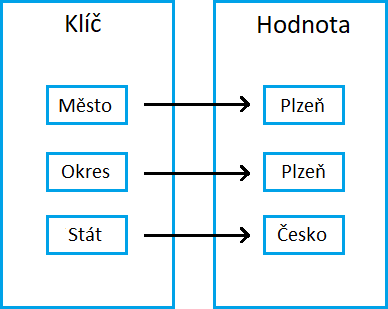
\includegraphics[width=10cm]{img/databaze/keyvalue_db}
	\caption{Ukázka databáze klíč-hodnota.}
	\label{fig:db_img_keyvalue}
	\end{figure}
\subsection{Grafová databáze}
Grafová databáze je typem NoSQL databáze, která je založená na teorii grafů. Data jsou reprezentována jako uzly, hrany zase reprezentují vztahy mezi daty. Graf lze procházet podél určitých typů hran nebo přes celý graf. Procházení spojení nebo relací je velmi rychlé, protože vztahy mezi uzly se nepočítají v době dotazu, ale jsou v databázi trvalé. Typické příklady jsou: Neo4j, OrientDB, Microsoft Azure CosmosDB. Ukázku grafové databáze lze vidět na obrázku č. \ref{fig:db_img_graph}.
	\begin{figure}[H]
	\centering
	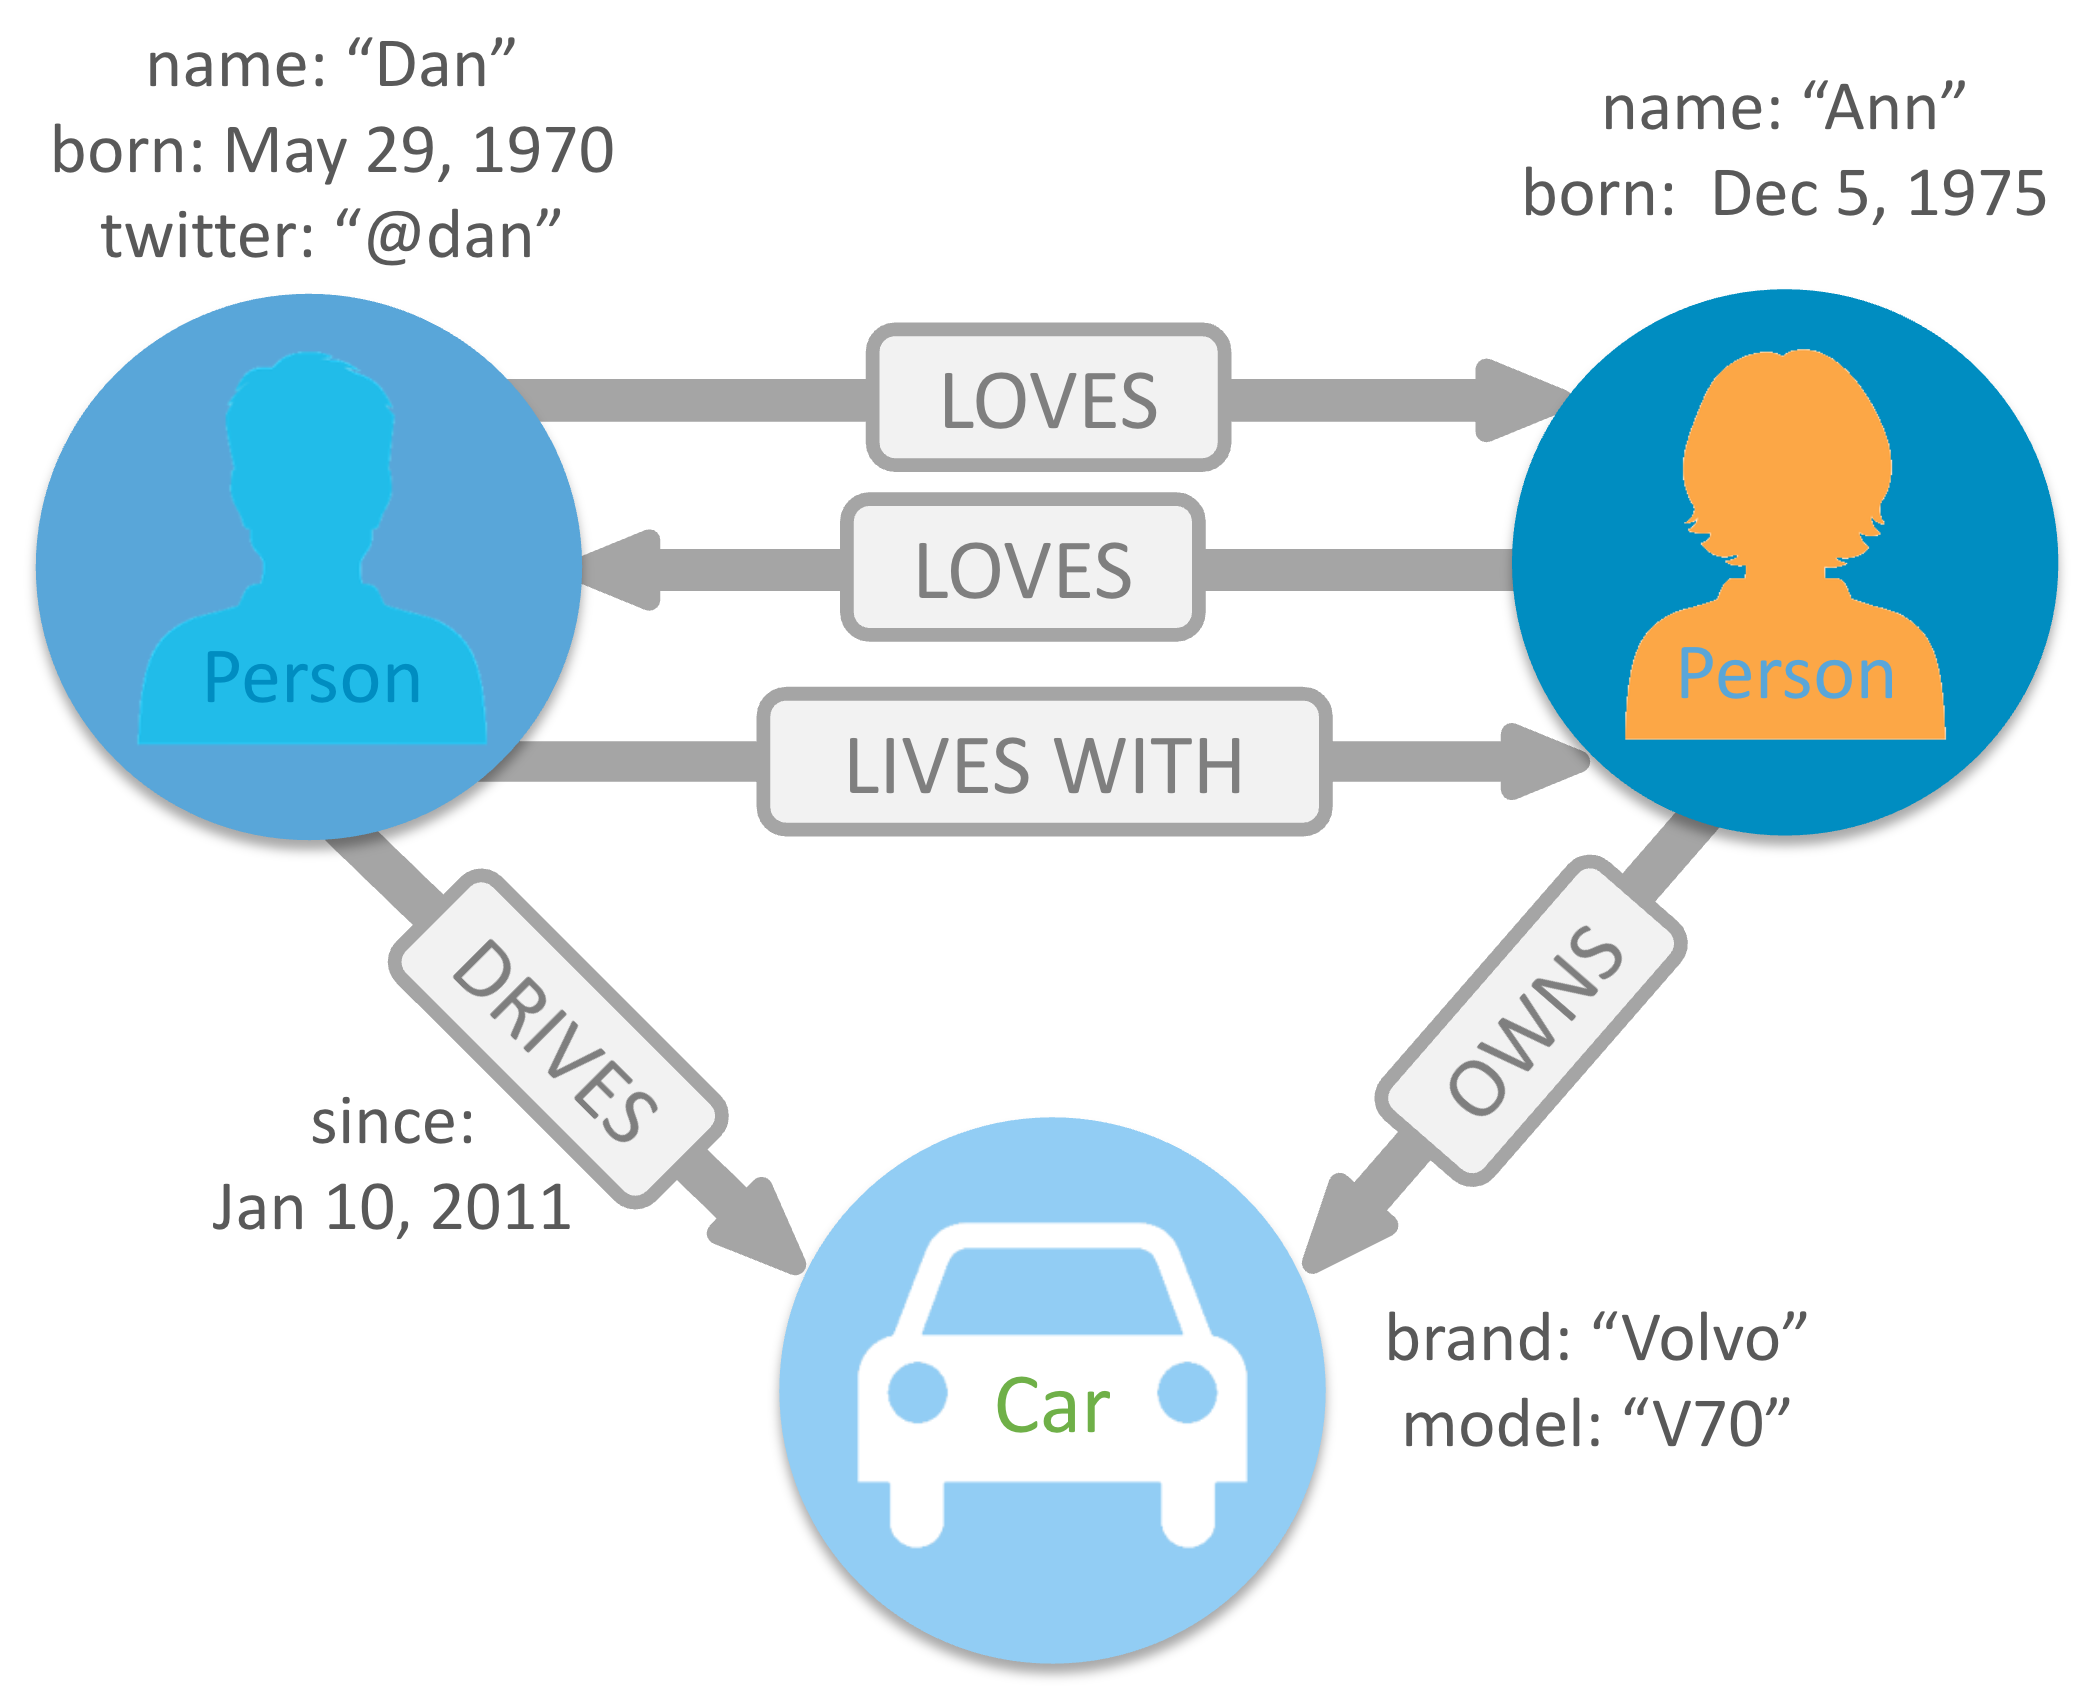
\includegraphics[width=8cm]{img/databaze/graph_db}
	\caption{Ukázka grafové databáze}
	\label{fig:db_img_graph}
	\end{figure}
\subsection{Dokumentová databáze}
Databáze dokumentů jsou typem NoSQL databáze a  jsou navržené pro ukládání, načítání a správu informací orientovaných na dokumenty. Dokumenty jsou obvykle uloženy ve formátu \gls{XML}, \gls{JSON}, \gls{BSON}. 
Typické příklady jsou: MongoDB, Amazon DocumentDB, Apache CouchDB. Ukázku dokumentové databáze lze vidět na obrázku č. \ref{fig:db_img_document}.
	\begin{figure}[H]
	\centering
	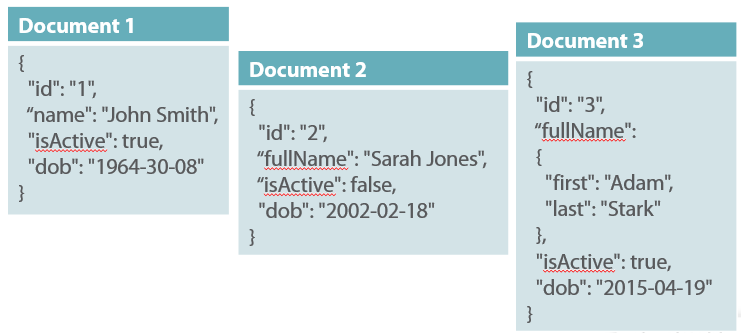
\includegraphics[width=11cm]{img/databaze/document_db}
	\caption{Ukázka dokumentově orientované databáze}
	\label{fig:db_img_document}
	\end{figure}
\subsection{Hierarchická databáze}
Hierarchická databáze používají k ukládání dat model nadřazený-podřízený, který představuje data ve stromové podobě. Vztah mezi záznamy je jeden k mnoha. To znamená, že jeden nadřazený uzel může mít mnoho podřízených, zatímco podřízený má vždy pouze jednoho nadřízeného.Typické příklady jsou: IBM Information Management System (IMS), RDM Mobile, Registry ve windows. Ukázku hierarchické databáze lze vidět na obrázku č. \ref{fig:db_img_hierarchical}.
	\begin{figure}[H]
	\centering
	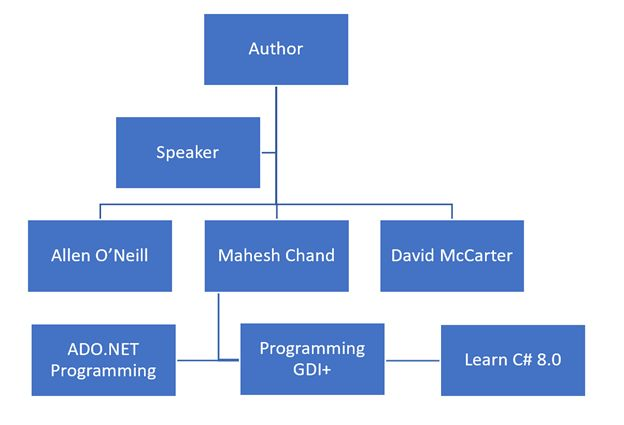
\includegraphics[width=9cm]{img/databaze/hierarchical_db}
	\caption{Ukázka hierarchické databáze}
	\label{fig:db_img_hierarchical}
	\end{figure}
%%%%%%%%%%%%%%%%%%%%%%%%%%%%%%%%%%%%%%%%%%%%%%%%%%%%%%%%%%%%

%\chapter{Docker}
%\todo{todo}
%Popsat docker jako takový - kontejnery, image, docker compose, ...\newline
%\section{Kontejner vs Virtuální stroj}